\chapter{Introduzione}
Il progetto vuole modellare e implementare un sistema in Java che permetta di generare tracce di un'esecuzione a partire dalla definizione di un taskset con o senza risorse da usare in mutua esclusione. Le eventuali risorse sono gestite da un protocollo di accesso alle risorse.

Ogni traccia è definita come una sequenza di coppie $<tempo, evento>$, dove un $evento$ può essere: rilascio di un job di un task; acquisizione/rilascio di un semaforo da parte di un job di un task; completamento di un chunk; completamento di un job di un task; preemption che un task può subire.

%%%%%%%%%%%%%%%%%%%%%%%%%%%%%%%%%%%%%%%%%%%%%%%%%%%%%%%%%%%%%%%%
\section{Capacità}
A partire da un taskset, il sistema ha le capacità di:
\begin{itemize}
    \item Generare la traccia di esecuzione del taskset schedulato tramite un dato algoritmo di scheduling (i.e., Rate Monotonic e Earlist Deadline First) e ed un eventuale protocollo di accesso alle risorse (i.e., Priority Ceiling Protocol). Considerando la gestione dinamica delle priorità da parte di EDF, è previsto il suo utilizzo solo senza risorse condivide.
    \item Generare un dataset di tracce relative a più simulazioni su un taskset.
    \item Specificare il tempo desiderato della simulazione.
    \item Rilevare eventuali deadline miss. Se un task non ha finito di eseguire entro la propria deadline allora la simulazione si arresta; non continua perché ci interessa valutare il primo fallimento, visto che i successivi potrebbero essere in cascata del primo.
    \item Introdurre e rilevare un additional execution time in un chunk. Questo modella un tempo di computazione di un chunk maggiore (o minore) di quello che ci aspettiamo, cioè maggiore del WCET.
    \item Introdurre un fault a livello del protocollo di accesso alle risorse (i.e., PCP) tale per cui la priorità dinamica assegnata al task che entra in critical section è quella corretta più un valore campionato da una distribuzione uniforme.
    \item Introdurre un fault a livello di chunk tale per cui con una certa probabilità il chunk non acquisisce, e quindi non rilascia, il semaforo che gestisce la risorsa associata alla critical section in cui entra.
\end{itemize}

%%%%%%%%%%%%%%%%%%%%%%%%%%%%%%%%%%%%%%%%%%%%%%%%%%%%%%%%%%%%%%%%
\section{Utilizzo}
Nei prossimi punti vediamo degli accorgimenti che sono utili per far utilizzare il sistema nel modo corretto.
\begin{itemize}
    \item Gli elementi del sistema, come chunk, task, taskset, scheduler e protocollo di accesso alle risorse, devono essere definiti all'interno del main. Una volta definito tutto si deve chiamare il metodo \texttt{schedule} sullo scheduler. Nel caso si voglia generare una sorta di dataset di tracce, è prevista la possibilità di chiamare più volte il medtodo \texttt{schedule} all'interno dello stesso main.
    \item Un chunk campiona il suo tempo di esecuzione da una distribuzione. Tale distribuzione, passata come parametro del costruttore, è un oggetto di tipo \texttt{Sampler} definito nella libreria Sirio. Oltre alle distribuzioni introdotte da Sirio è presente anche l'implementazione \texttt{ConstantSampler}, che definisce un campionamento costante.
    \item I tempi devono essere passati al sistema e letti da esso in milli secondi. Il sistema li gestisce in nanosecondi per avere un'alta precisione.
    \item Quando si vuole introdurre il fault relativo alla priorità dinamica settata da PCP si deve specificare il valore minimo e massimo entro cui campionare. Questi valori sono intesi come esclusi.
    \item Quando si vuole introdurre il fault relativo all'acquisizione del semafore associato alle risorse, la soglia specificata deve essere in un intervallo 0.0 e 1.0.
\end{itemize}

\subsection{Esempio 1}
Nella Figura~\ref{fig:esempioRM} vediamo un esempio di simulazione di RM per generare un dataset di tracce su un taskset.
\begin{figure}[htbp]
    \centering
    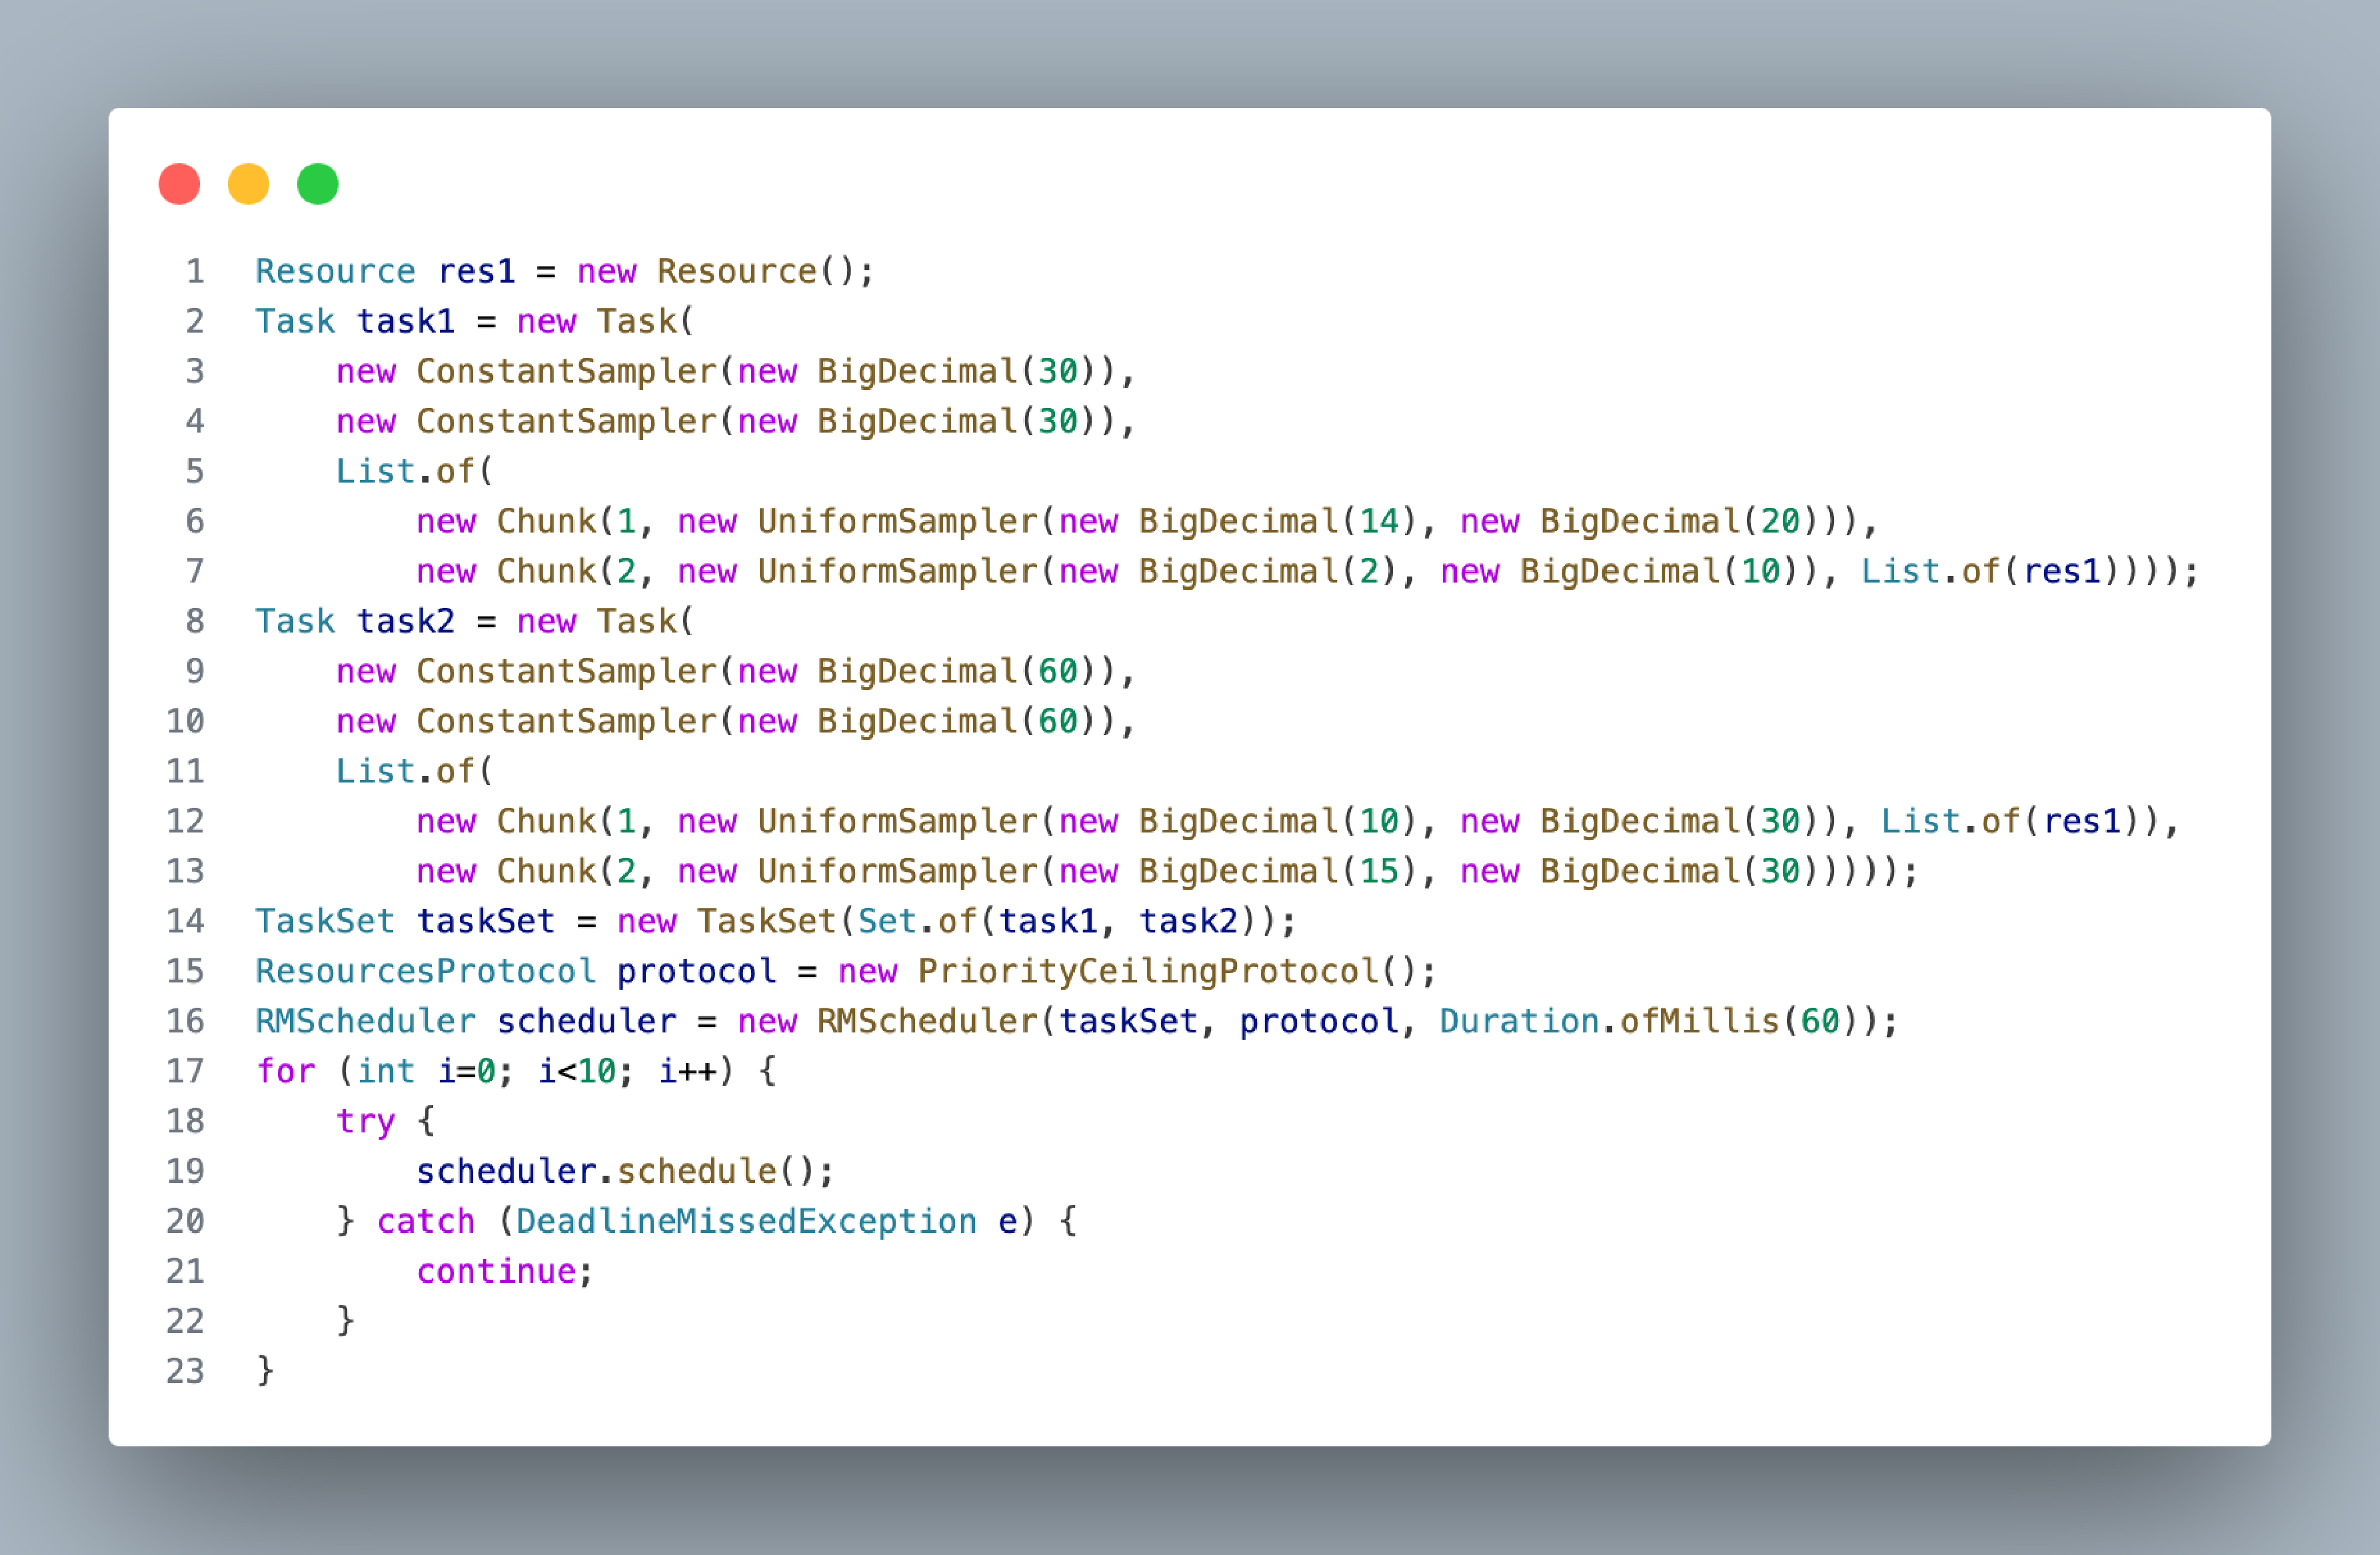
\includegraphics[width=.5\textwidth]{immagini/esempio RM con risorse.pdf}
    \caption{Esempio RM con PCP.}
    \label{fig:esempioRM}
\end{figure}

\subsection{Esempio 2}
Nella Figura~\ref{fig:esempioRMConFault} vediamo un esempio di simulazione di RM per generare un dataset di tracce su un taskset i cui task utilizzano risorse condivise.
\begin{figure}[htbp]
    \centering
    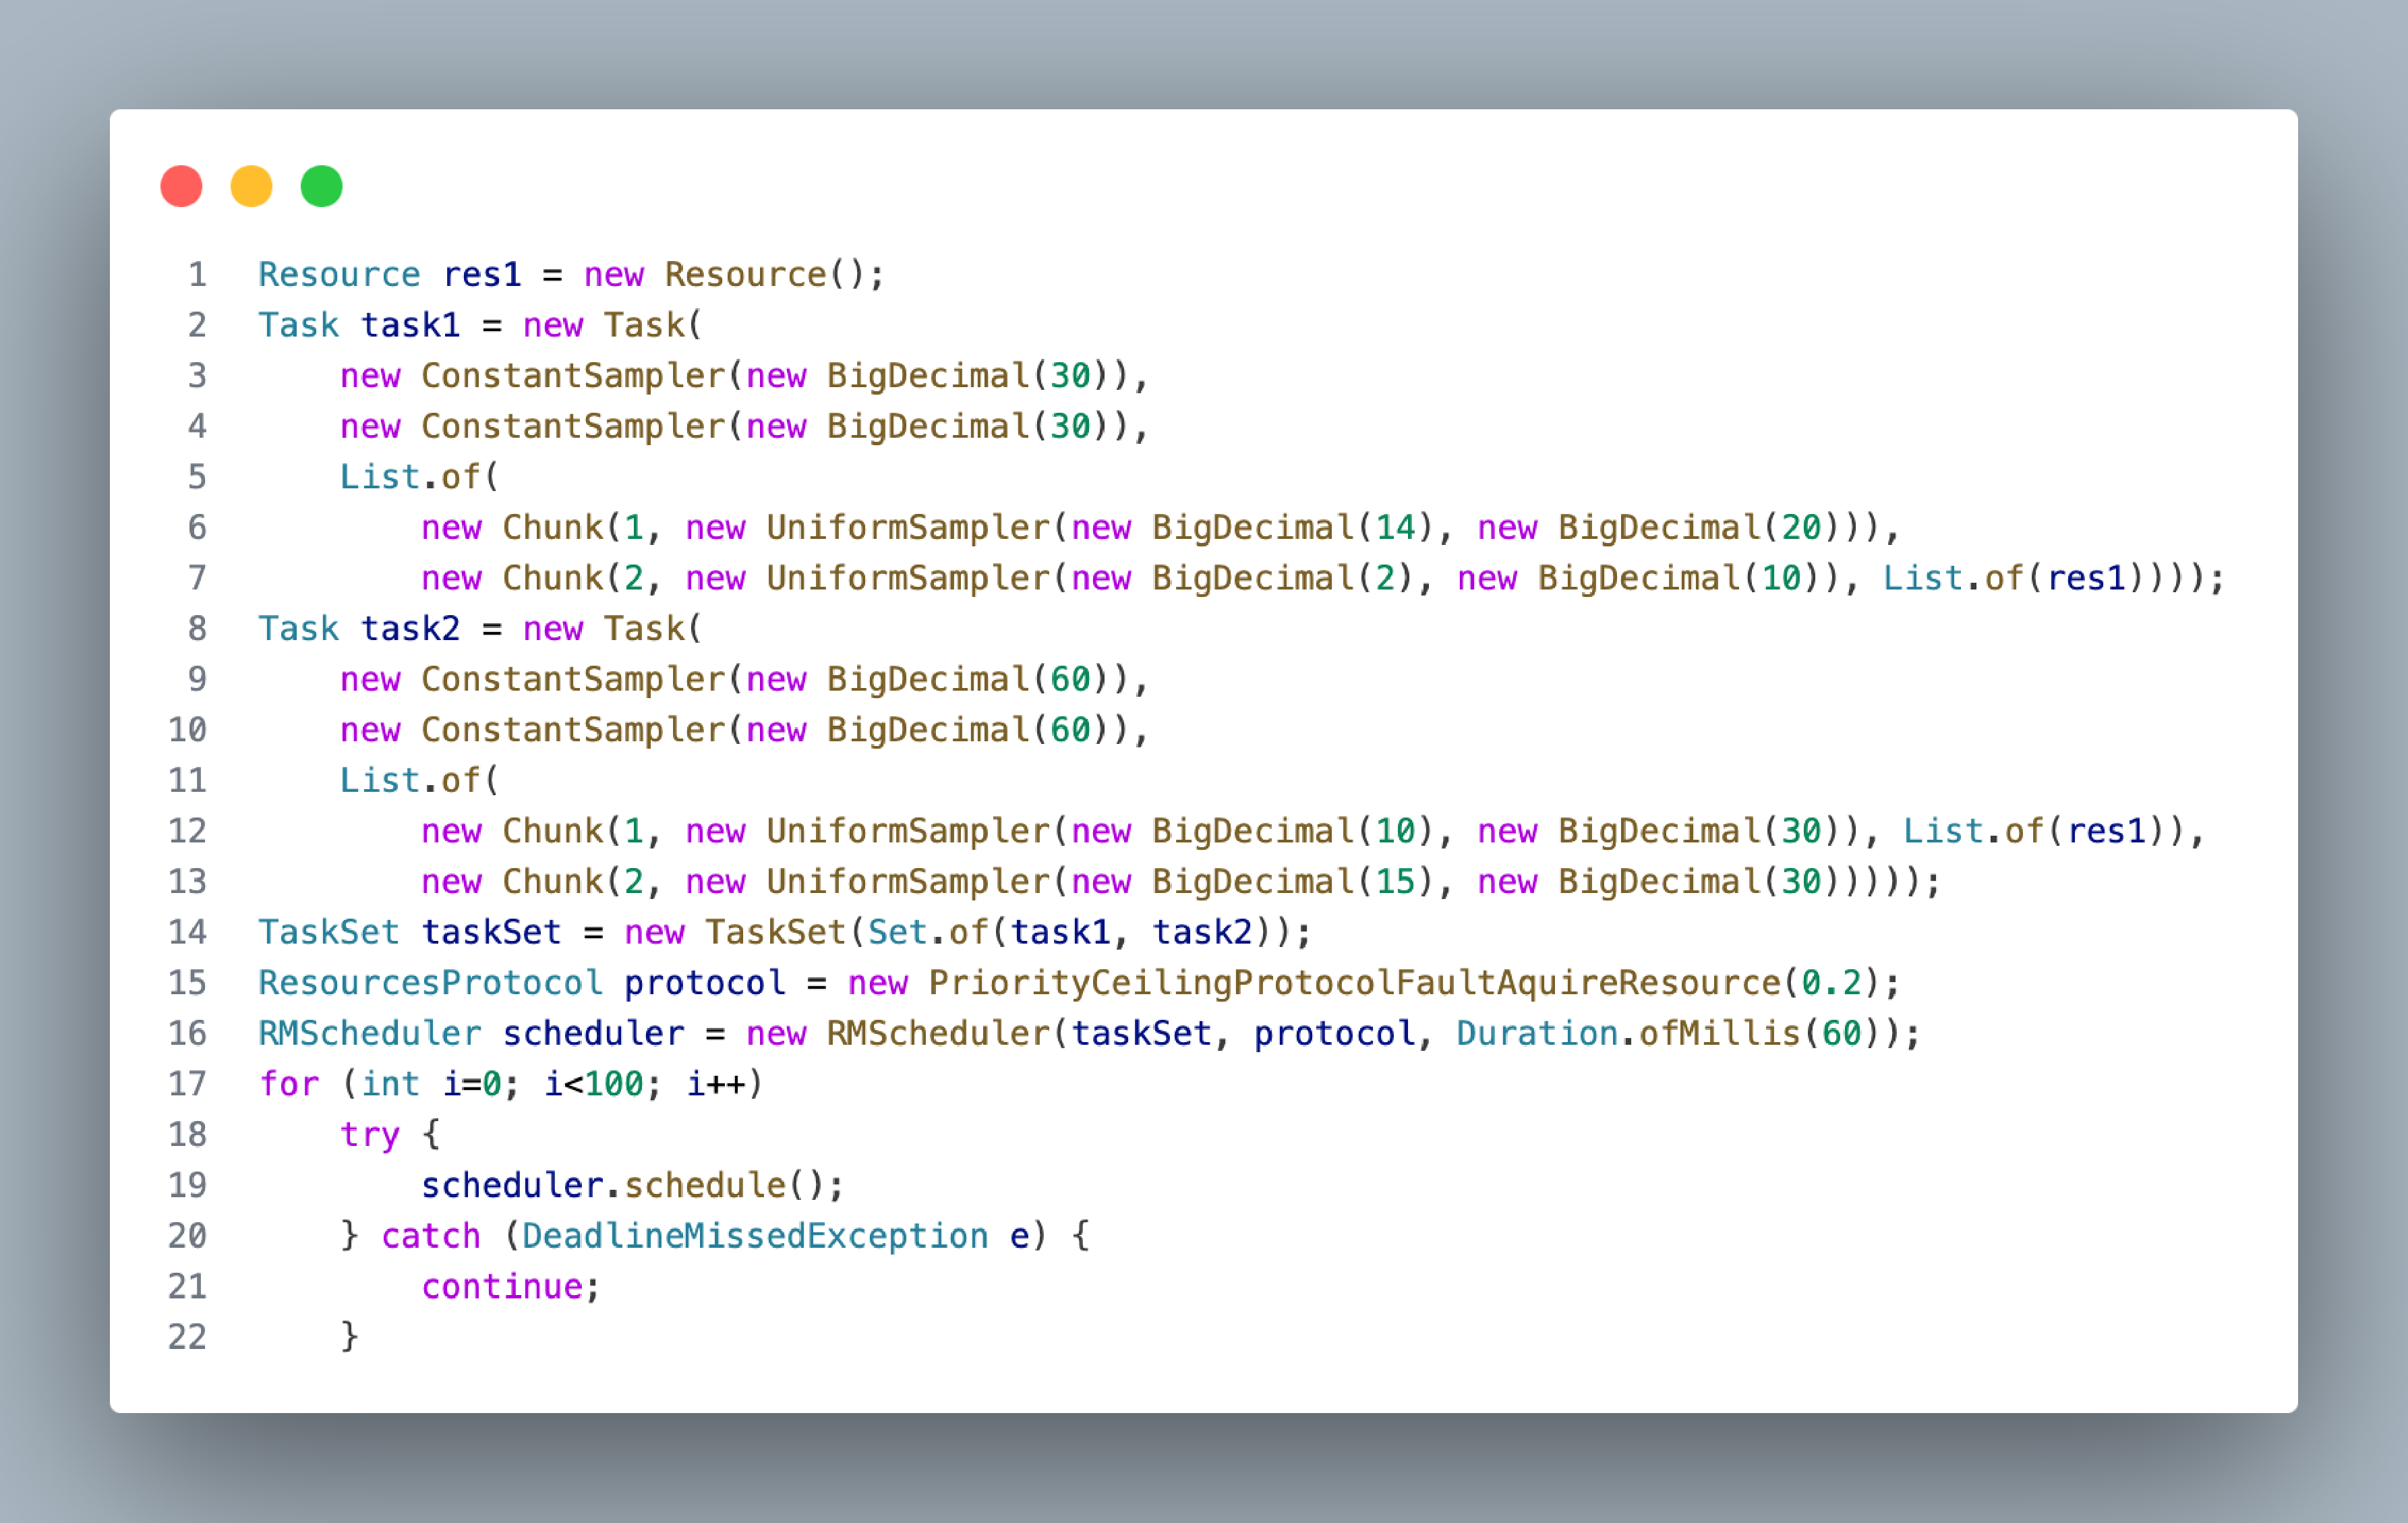
\includegraphics[width=.5\textwidth]{immagini/esempio RM con fault.pdf}
    \caption{Esempio RM con PCP.}
    \label{fig:esempioRMConFault}
\end{figure}